%---------------------------------------------------------%
\section{The $\bP^1_{nc}-P^0_{Mps}$ scheme}\label{sec:MPFA}

Here, we use the symmetric MPFA scheme (where MPFA stands for {\em multi-points flux approximation}) to discretize the pressure gradient term in \eqref{eq:Stokes}, in the case of a simplicial mesh. The discrete pressure space remains $Q_h=Q_{0,h}$. We call this new scheme the $\bP^1_{nc}-P^0_{Mps}$ scheme.
\par
Let us consider the $2D$ case.
To design the scheme, as it has been initially done in \cite{LEPOTIER05bis, LEPOTIER05}, we start by splitting the triangles into three quadrangles, connecting the barycentre of the triangle to the midpoint of each edges. Considering some $ q_h \in Q_h$, we will calculate an affine approximation of $Q_h$ on each quadrangles. To do so,we need to add temporary auxiliary unknowns located on the third of the edges.
\\
%-----------------------------------------%
%\subsection{Notations and dual mesh in $2D$}
%-----------------------------------------%
Let us introduce some notations. \\

Let  $j \in \Ical_{S}$. We define the macro-element $\Mcal_j$ such that $\ds\overline{\Mcal}_j:=\bigcap_{\ell\in\Ical_{K,j}}\overline{K}_\ell$. Let renumber the vertices so that: $S_0=S_j$, $\Ical_{S,0}=\{1,\cdots,N_{S,0}\}$ and for all $i\in\Ical_{S,0}$, $S_iS_{i+1}\in\Fcal_h$ (setting $S_{N_{S,0}+1}=S_{N_{S,0}}$). For $i\in\Ical_{S,0}$ we denote by:
\begin{itemize}
	\item $K_i$ the triangle of vertices $S_0 S_i S_{i+1}$, and we call its barycentre $G_i$.
	\item $F_i$ the edge such that $F_i=S_0S_i$, and we call $M_i$ its midpoint. 
	\item $F_{i,0}$ the edge opposite to $S_0$ in $K_i$. 
	\item $\tilde{F}_i$ the half-edges defined by $S_0$ and the midpoint of $F_i$.
	\item $Q_i$ the quadrangle of vertices $S_0\,M_i\,G_i\,M_{i+1}$ (Fig. \ref{fig:Qi}-(a) for $S_0\in\Om$ and \ref{fig:Qj}-(a) for $S_0\in\pa\Om$).
\end{itemize}
For $i,\,j\in\Ical_{S,0}$, we denote by $\Scal_{i,j}$ the normal vector outgoing of $K_j$ at $F_i$ and of norm $|F_i|$. For $i\in\Ical_{S,0}$, we call $\Scal_{0,i}$ the normal vector outgoing of $K_i$ at $F_{i,0}$. On Figure \ref{fig:MS_and_T1}-(a), we represent $\Mcal_0$ in case $S_0\in\Om$ and $N_{S,0}=6$. On Figure \ref{fig:MS_and_T1}-(b), we represent the triangle $K_1$ with the vectors $(\Scal_{j,1})_{j=0}^2$ and its barycentre $G_1$.
\vspace{-0.3cm}
\begin{center}
	\begin{figure}[ht!]
		\begin{subfigure}[b]{0.39\linewidth}
			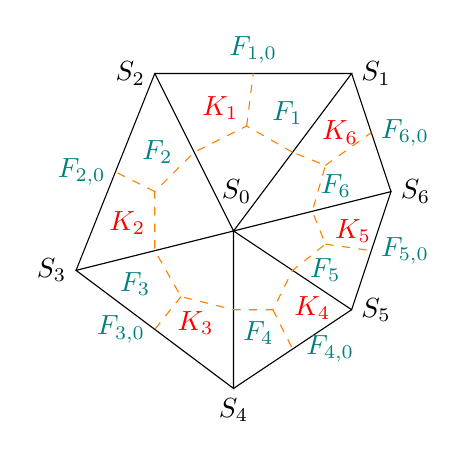
\begin{tikzpicture}[scale=0.5]
			% triangles
			\draw[-] (0,0) -- (3,4) -- (-2,4) --cycle;
			\draw[-] (0,0) -- (-4,-1) -- (0,-4) --cycle;
			\draw[-] (0,0) -- (3,-2) -- (4,1) --cycle;
			\draw[-] (-4,-1) -- (-2,4);
			\draw[-] (0,-4) -- (3,-2);
			\draw[-] (4,1) -- (3,4);
			%quadriangle
			\draw[dashed,orange] (1.5,2)--(1/3,8/3)--(-1,2)--(-2,1)--(-2,-0.5)--(-4/3,-5/3)--(0,-2)--(1,-2)--(1.5,-1)--(7/3,-1/3)--(2,0.5)--(7/3,5/3)--(1.5,2);
			\draw[dashed,orange] (1/3,8/3)--(1/2,8/2);
			\draw[dashed,orange] (-2,1)--(-3,3/2);
			\draw[dashed,orange] (-4/3,-5/3)--(-4/2,-5/2);
			\draw[dashed,orange] (1,-2)--(3/2,-3);
			\draw[dashed,orange] (7/3,-1/3)--(7/2,-1/2);
			\draw[dashed,orange] (7/3,5/3)--(7/2,5/2);
			
			% sommets
			\coordinate [label=left:$S_0$] (S_0) at (0.7,1);
			\coordinate [label=right:$S_1$] (S1) at (3,4);
			\coordinate [label=left:$S_2$] (S2) at (-2,4);
			\coordinate [label=left:$S_3$] (S3) at (-4,-1);
			\coordinate [label=below:$S_4$] (S4) at (0,-4);
			\coordinate [label=right:$S_5$] (S5) at (3,-2);
			\coordinate [label=right:$S_6$] (S6) at (4,1);
			% faces
			\coordinate [label=above:\textcolor{teal}{$F_{1,0}$}] (F1) at (1/2,4);
			\coordinate [label=left:\textcolor{teal}{$F_{2,0}$}] (F1) at (-3,1.5);
			\coordinate [label=left:\textcolor{teal}{$F_{3,0}$}] (F1) at (-2,-2.5);
			\coordinate [label=right:\textcolor{teal}{$F_{4,0}$}] (F1) at (1.6,-3);
			\coordinate [label=right:\textcolor{teal}{$F_{5,0}$}] (F1) at (3.5,-0.5);
			\coordinate [label=right:\textcolor{teal}{$F_{6,0}$}] (F1) at (3.5,2.5);
			\coordinate [label=left:\textcolor{teal}{$F_1$}] (F1) at (2,3);
			\coordinate [label = left:\textcolor{teal}{$F_2$}] (F2) at (-1.3,2);
			\coordinate [label=below:\textcolor{teal}{$F_3$}] (F3) at (-2.5,-0.8);
			\coordinate [label=right:\textcolor{teal}{$F_4$}] (F4) at (0,-2.6);
			\coordinate [label=right:\textcolor{teal}{$F_5$}] (F5) at (1.7,-1);
			\coordinate [label=above:\textcolor{teal}{$F_6$}] (F6) at (2.6,0.6);
			% Triangles
			\coordinate [label=below:\textcolor{red}{$K_1$}] (T1) at (-1/3,11/3);
			\coordinate [label=right:\textcolor{red}{$K_2$}] (T2) at (-3.4,0.2);
			\coordinate [label=right:\textcolor{red}{$K_3$}] (T3) at (-5/3,-7/3);
			\coordinate [label=above:\textcolor{red}{$K_4$}] (T4) at (2,-2.5);
			\coordinate [label=right:\textcolor{red}{$K_5$}] (T5) at (7/3,-0);
			\coordinate [label=right:\textcolor{red}{$K_6$}] (T6) at (6/3,2.5);
			\end{tikzpicture}
			\caption{Macro-element $\Mcal_0=S_1\,S_2\,S_3\,S_4\,S_5\,S_6$.}
		\end{subfigure}
		\hspace{0.2\linewidth}
		\begin{subfigure}[b]{0.39\linewidth}
			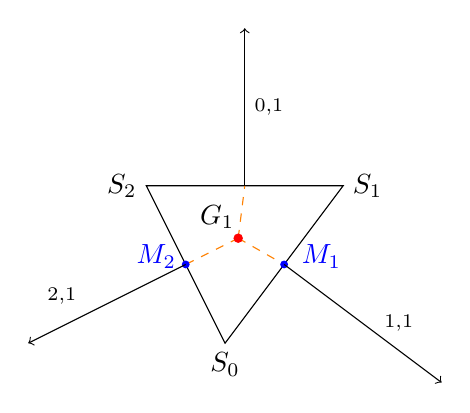
\begin{tikzpicture}[scale=0.5]
			=% triangle
			\draw[-] (0,0) -- (3,4) -- (-2,4) --cycle;
			% sommets
			\coordinate [label=below:$S_0$] (S) at (0,0);
			\coordinate [label=right:$S_1$] (S1) at (3,4);
			\coordinate [label=left:$S_2$] (S2) at (-2,4);
			% quadrangle 
			\draw[dashed,orange] (1/3,8/3)--(1.5,2);
			\draw[dashed,orange] (1/3,8/3)--(-1,2.0);
			\draw[dashed,orange] (1/3,8/3)--(1/2,4);
			% milieux des faces
			\fill[fill=blue] (-1,2) circle (0.1cm);
			\coordinate [label=left:\textcolor{blue}{$M_2$}] (M2) at (-1,2.2);
			\fill[fill=blue] (1.5,2) circle (0.1cm);
			\coordinate [label=right:\textcolor{blue}{$M_1$}] (M1) at (1.7,2.2);
			% barycentre
			\coordinate [label = above:$G_1$] (G) at (-1/5,8/3);
			\fill[fill=red] (1/3,8/3) circle (0.12cm);
			\draw [->] (1.5,2) --(5.5,-1);
			\coordinate [label = right:$\Scal_{1,1}$] (N1) at (3.8,0.5);
			\draw [->] (-1,2) -- (-5,0);
			\coordinate [label = left:$\Scal_{2,1}$] (N2) at (-3.5,1.2);
			\draw [->] (0.5,4) -- (0.5,8);
			\coordinate [label = right:$\Scal_{0,1}$] (N0) at (0.5,6);
			\end{tikzpicture}
			\caption{Triangle $K_1=S_0\,S_1\,S_2$.}
		\end{subfigure}
		\caption{Notations in case $N_{S,0}=6$ and $j\in \Ical_S^i$.}
		\label{fig:MS_and_T1}
	\end{figure}
\end{center}
\vspace{-1.1cm}
%----------------------------------------------------------%
%\subsection{Pressure gradient scheme around an inner vertex}
%----------------------------------------------------------% 
\begin{center}
	\begin{figure}[ht!]
		\begin{subfigure}[b]{0.39\linewidth}
			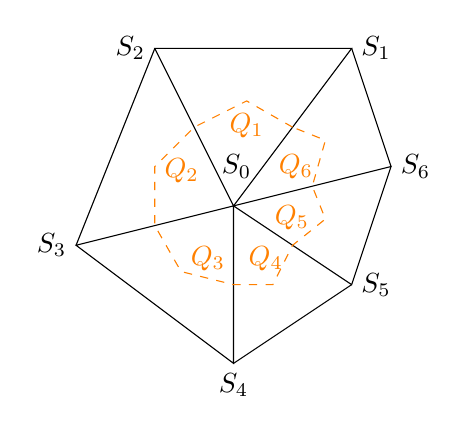
\begin{tikzpicture}[scale=0.5]
			% triangles
			\draw[-] (0,0) -- (3,4) -- (-2,4) --cycle;
			\draw[-] (0,0) -- (-4,-1) -- (0,-4) --cycle;
			\draw[-] (0,0) -- (3,-2) -- (4,1) --cycle;
			\draw[-] (-4,-1) -- (-2,4);
			\draw[-] (0,-4) -- (3,-2);
			\draw[-] (4,1) -- (3,4);
			% quadrangles
			\draw[dashed,orange] (1.5,2)--(1/3,8/3)--(-1,2)--(-2,1)--(-2,-0.5)--(-4/3,-5/3)--(0,-2)--(1,-2)--(1.5,-1)--(7/3,-1/3)--(2,0.5)--(7/3,5/3)--(1.5,2);
			% sommets
			\coordinate [label=left:$S_0$] (S) at (0.7,1);
			\coordinate [label=right:$S_1$] (S1) at (3,4);
			\coordinate [label=left:$S_2$] (S2) at (-2,4);
			\coordinate [label=left:$S_3$] (S3) at (-4,-1);
			\coordinate [label=below:$S_4$] (S4) at (0,-4);
			\coordinate [label=right:$S_5$] (S5) at (3,-2);
			\coordinate [label=right:$S_6$] (S6) at (4,1);
			%
			% quadrangles
			\coordinate [label=below:\textcolor{orange}{$Q_1$}] (Q1) at (1/3,7.8/3);
			\coordinate [label=right:\textcolor{orange}{$Q_2$}] (Q2) at (-2,0.9);
			\coordinate [label=right:\textcolor{orange}{$Q_3$}] (Q3) at (-4/3,-4/3);
			\coordinate [label=above:\textcolor{orange}{$Q_4$}] (Q4) at (0.82,-1.9);
			\coordinate [label=right:\textcolor{orange}{$Q_5$}] (Q5) at (0.80,-0.30);
			\coordinate [label=right:\textcolor{orange}{$Q_6$}] (Q6) at (0.90,1);
			\end{tikzpicture}
			\caption{Quadrangles $(Q_i)_{i=1}^{N_{S,0}}$.}
		\end{subfigure}
		\hspace{0.2\linewidth}
		\begin{subfigure}[b]{0.39\linewidth} 
			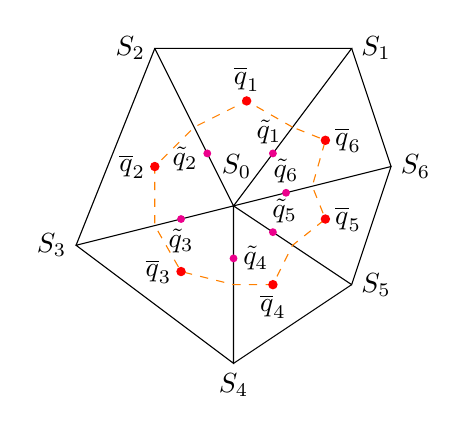
\begin{tikzpicture}[scale=0.5]
			% triangles
			\draw[-] (0,0) -- (3,4) -- (-2,4) --cycle;
			\draw[-] (0,0) -- (-4,-1) -- (0,-4) --cycle;
			\draw[-] (0,0) -- (3,-2) -- (4,1) --cycle;
			\draw[-] (-4,-1) -- (-2,4);
			\draw[-] (0,-4) -- (3,-2);
			\draw[-] (4,1) -- (3,4);
			% quadrangles
			\draw[dashed,orange] (1.5,2)--(1/3,8/3)--(-1,2)--(-2,1)--(-2,-0.5)--(-4/3,-5/3)--(0,-2)--(1,-2)--(1.5,-1)--(7/3,-1/3)--(2,0.5)--(7/3,5/3)--(1.5,2);
			% sommets
			\coordinate [label=left:$S_0$] (S) at (0.7,1);
			\coordinate [label=right:$S_1$] (S1) at (3,4);
			\coordinate [label=left:$S_2$] (S2) at (-2,4);
			\coordinate [label=left:$S_3$] (S3) at (-4,-1);
			\coordinate [label=below:$S_4$] (S4) at (0,-4);
			\coordinate [label=right:$S_5$] (S5) at (3,-2);
			\coordinate [label=right:$S_6$] (S6) at (4,1);
			%
			% Barycentres
			\coordinate [label = above:$\overline{q}_1$] (pT1) at (1/3,8/3);
			\fill[fill=red] (1/3,8/3) circle (0.12cm);
			\coordinate [label = left:$\overline{q}_2$] (pT2) at (-2,1);
			\fill[fill=red] (-2,1) circle (0.12cm);
			\coordinate [label = left:$\overline{q}_3$] (pT3) at (-4/3,-5/3);
			\fill[fill=red] (-4/3,-5/3) circle (0.12cm);
			\coordinate [label = below:$\overline{q}_4$] (pT4) at (1,-2) ;
			\fill[fill=red] (1,-2) circle (0.12cm);
			\coordinate [label = right:$\overline{q}_5$] (pT5) at (7/3,-1/3) ;
			\fill[fill=red] (7/3,-1/3) circle (0.12cm);
			\coordinate [label = right:$\overline{q}_6$] (pT6) at (7/3,5/3) ;
			\fill[fill=red] (7/3,5/3) circle (0.12cm);
			% pressions auxiliaires
			\coordinate [label = above:$\tilde{q}_1$] (p1) at (0.9,4/3);
			\fill[fill=magenta] (1,4/3) circle (0.1cm);
			\coordinate [label = left:$\tilde{q}_2$] (p2) at (-2/3,1.2);
			\fill[fill=magenta] (-2/3,4/3) circle (0.1cm);
			\coordinate [label = below:$\tilde{q}_3$] (p3) at (-4/3,-1/3);
			\fill[fill=magenta] (-4/3,-1/3) circle (0.1cm);
			\coordinate [label = right:$\tilde{q}_4$] (p4) at (0,-4/3);
			\fill[fill=magenta] (0,-4/3) circle (0.1cm);
			\coordinate [label = above:$\tilde{q}_5$] (p5) at (1.3,-0.68);
			\fill[fill=magenta] (1,-2/3) circle (0.1cm);
			\coordinate [label = above:$\tilde{q}_6$] (p6) at (4/3,1/3);
			\fill[fill=magenta] (4/3,1/3) circle (0.1cm);
			
			\end{tikzpicture}
			\caption{Discrete pressures ($\overline{q}_i$,$\tilde{q}_i)_{i=1}^{N_{S,0}}$.}
		\end{subfigure}
		\caption{MPFA Scheme for $j \in \Ical_S^i$ and $N_{S,0}=6$.}
		\label{fig:Qi}
	\end{figure}
\end{center}
\begin{center}
	\begin{figure}[h]
		\begin{subfigure}[b]{0.39\linewidth}
			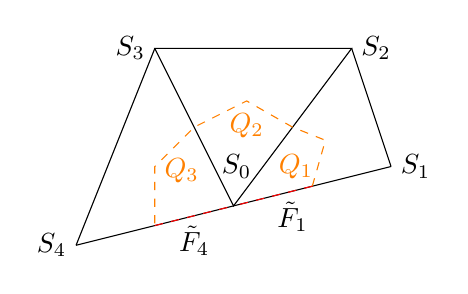
\begin{tikzpicture}[scale=0.5]
			% triangles
			\draw[-] (0,0) -- (3,4) -- (-2,4) --cycle;
			%			\draw[-] (0,0) -- (-4,-1) -- (0,-4) --cycle;
			%			\draw[-] (0,0) -- (3,-2) -- (4,1) --cycle;
			\draw[-] (-4,-1) -- (-2,4);
			%			\draw[-] (0,-4) -- (3,-2);
			\draw[-] (-4,-1) -- (4,1);
			\draw[-] (4,1) -- (3,4);
			% quadrangles
			\draw[dashed,orange] (1.5,2)--(1/3,8/3)--(-1,2)--(-2,1)--(-2,-0.5);
			\draw[dashed,orange] (2,0.5)--(7/3,5/3)--(1.5,2);
			% sommets
			\coordinate [label=left:$S_0$] (S) at (0.7,1);
			\coordinate [label=right:$S_2$] (S2) at (3,4);
			\coordinate [label=left:$S_3$] (S3) at (-2,4);
			\coordinate [label=left:$S_4$] (S4) at (-4,-1);
			%			\coordinate [label=below:$S_4$] (S4) at (0,-4);
			%			\coordinate [label=right:$S_5$] (S5) at (3,-2);
			\coordinate [label=right:$S_1$] (S1) at (4,1);
			%
			% quadrangles
			\coordinate [label=below:\textcolor{orange}{$Q_2$}] (Q2) at (1/3,7.8/3);
			\coordinate [label=right:\textcolor{orange}{$Q_3$}] (Q3) at (-2,0.9);
			%			\coordinate [label=right:\textcolor{orange}{$Q_3$}] (Q3) at (-4/3,-4/3);
			%			\coordinate [label=above:\textcolor{orange}{$Q_4$}] (Q4) at (0.82,-1.9);
			%			\coordinate [label=right:\textcolor{orange}{$Q_5$}] (Q5) at (0.80,-0.30);
			\coordinate [label=right:\textcolor{orange}{$Q_1$}] (Q1) at (0.90,1);
			% Demi-arêtes 
			\coordinate [label=below:$\tilde{F}_4$] (FI4) at (-1,-0.25);
			\coordinate [label=below:$\tilde{F}_1$] (FI1) at (6/4,0.35);
			\draw[dashed,red] (-2,-0.5)--(0,0);
			\draw[dashed,red] (2,0.5)--(0,0);
			\end{tikzpicture}
			\caption{Quadrangles $(Q_i)_{i=1}^{N_{S,0}}$.}
		\end{subfigure}
		\hspace{0.2\linewidth}
		\begin{subfigure}[b]{0.39\linewidth} 
			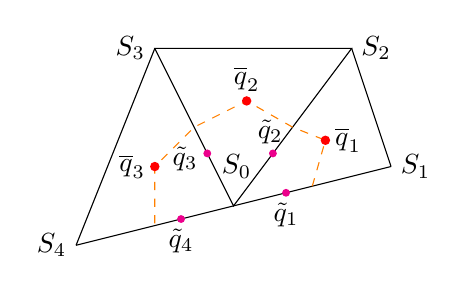
\begin{tikzpicture}[scale=0.5]
			% triangles
			\draw[-] (0,0) -- (3,4) -- (-2,4) --cycle;
			%			\draw[-] (0,0) -- (-4,-1) -- (0,-4) --cycle;
			%			\draw[-] (0,0) -- (3,-2) -- (4,1) --cycle;
			\draw[-] (-4,-1) -- (-2,4);
			%			\draw[-] (0,-4) -- (3,-2);
			\draw[-] (-4,-1) -- (4,1);
			\draw[-] (4,1) -- (3,4);
			% quadrangles
			\draw[dashed,orange] (1.5,2)--(1/3,8/3)--(-1,2)--(-2,1)--(-2,-0.5);
			\draw[dashed,orange] (2,0.5)--(7/3,5/3)--(1.5,2);
			% sommets
			\coordinate [label=left:$S_0$] (S) at (0.7,1);
			\coordinate [label=right:$S_2$] (S2) at (3,4);
			\coordinate [label=left:$S_3$] (S3) at (-2,4);
			\coordinate [label=left:$S_4$] (S4) at (-4,-1);
			%			\coordinate [label=below:$S_4$] (S4) at (0,-4);
			%			\coordinate [label=right:$S_5$] (S5) at (3,-2);
			\coordinate [label=right:$S_1$] (S1) at (4,1);
			%
			% Barycentres
			\coordinate [label = above:$\overline{q}_2$] (pT2) at (1/3,8/3);
			\fill[fill=red] (1/3,8/3) circle (0.12cm);
			\coordinate [label = left:$\overline{q}_3$] (pT3) at (-2,1);
			\fill[fill=red] (-2,1) circle (0.12cm);
			%			\coordinate [label = left:$\overline{p}_3$] (pT3) at (-4/3,-5/3);
			%			\fill[fill=red] (-4/3,-5/3) circle (0.12cm);
			%			\coordinate [label = below:$\overline{p}_4$] (pT4) at (1,-2) ;
			%			\fill[fill=red] (1,-2) circle (0.12cm);
			%			\coordinate [label = right:$\overline{p}_5$] (pT5) at (7/3,-1/3) ;
			%			\fill[fill=red] (7/3,-1/3) circle (0.12cm);
			\coordinate [label = right:$\overline{q}_1$] (pT1) at (7/3,5/3) ;
			\fill[fill=red] (7/3,5/3) circle (0.12cm);
			% pressions auxiliaires
			\coordinate [label = above:$\tilde{q}_2$] (p2) at (0.93,4/3);
			\fill[fill=magenta] (1,4/3) circle (0.1cm);
			\coordinate [label = left:$\tilde{q}_3$] (p3) at (-2/3,1.2);
			\fill[fill=magenta] (-2/3,4/3) circle (0.1cm);
			\coordinate [label = below:$\tilde{q}_4$] (p4) at (-4/3,-1/3);
			\fill[fill=magenta] (-4/3,-1/3) circle (0.1cm);
			%			\coordinate [label = right:$\tilde{p}_4$] (p4) at (0,-4/3);
			%			\fill[fill=magenta] (0,-4/3) circle (0.1cm);
			%			\coordinate [label = above:$\tilde{p}_5$] (p5) at (1,-2/3);
			%			\fill[fill=magenta] (1,-2/3) circle (0.1cm);
			\coordinate [label = below:$\tilde{q}_1$] (p1) at (4/3,1/3);
			\fill[fill=magenta] (4/3,1/3) circle (0.1cm);
			
			\end{tikzpicture}
			\caption{Discrete pressures ($\overline{q}_i$,$\tilde{q}_i)_{i=1}^{N_{S,0}}$.}
		\end{subfigure}
		\caption{MPFA Scheme for $j \in \Ical_S^b$ and $N_{S,0}=4$ }
		\label{fig:Qj}
	\end{figure}
\end{center}
\vspace{-0.5cm}
Let $q_h\in Q_h$. We set $q_{h|K_\ell}:=\ov{q}_\ell$.
\\
Consider $S_0\in\Om$ (Fig. \ref{fig:Qi}). Let us build a piecewise affine approximation of $q_h$ on each quadrangle $(Q_i)_{i=1}^{N_{S,0}}$ (see Fig. \ref{fig:Qi}-(a)). We call this approximation $\tilde{q}_h$. We first introduce auxiliary discrete pressure values $(\tilde{q}_i)_{i=1}^{N_{S,0}}$ on the thirds of the inner edges of $\Mcal_0$ (see Fig. \ref{fig:Qi}-(b)). For all $j\in\Ical_{S,i}$, we define $\Gcal_i(q_h):=\grad\tilde{q}_{h|Q_i}$, using an integration by part as it is done in \cite[Sect. 3]{LEPOTIER05bis} and \cite[Sect. 1.1.1]{lepotierhdr}: % $\ds\frac{\Scal_{i,i+1}}{d}$: 
$$ |Q_i| \Gcal_i= \int_{Q_i} \Gcal_i(q_h) = \int_{\partial Q_i} \tilde{q}_h  \nvec_{\partial Q_i}=\, \tilde{q}_i \frac{\Scal_{i,i}}{d} + \tilde{q}_{i+1}\,\frac{\Scal_{i+1,i}}{d}  + \ov{q}_i(-\frac{\Scal_{i,i}}{d}-\frac{\Scal_{i+1,i}}{d}). $$ 


Hence, noticing that $|Q_i|= \frac{|T_i|}{d+1}$, we have:
\begin{equation}\label{eq:gradientlocal1}
\Gcal_i(q_h)=\ds\frac{1}{|Q_i|}\left(\,(\tilde{q}_i-\ov{q}_i)\,\frac{\Scal_{i,i}}{d}+(\tilde{q}_{i+1}-\ov{q}_i)\,\frac{\Scal_{i+1,i}}{d}\right) =\ds\frac{d+1}{d\,|T_i|}\left(\,\tilde{q}_i\,\Scal_{i,i}+\tilde{q}_{i+1}\,\Scal_{i+1,i}+\ov{q}_i\,\Scal_{0,i}\,\right).
\end{equation}
In order to preserve the flux across the inner edges of $\Mcal_0$, we write that:
%--------------%
\begin{equation}\label{eq:continuitefacesnormales}
\forall i\in\Ical_{S,0},\quad \Gcal_i(q_h)\cdot\Scal_{i+1,i}+\Gcal_{i+1}(q_h)\cdot\Scal_{i+1,i+1}=0.
\end{equation}
These $N_{S,0}$ equations with $N_{S,0}$ unknowns (the auxiliary discrete pressure values $(\tilde{q}_i)_{i=1}^{N_{S,0}}$) lead to a well posed linear system. Thus, we can evaluate the auxiliary discrete pressure values $(\tilde{q}_i)_{i=1}^{N_{S,0}}$ with the data $(\ov{q}_i)_{i=1}^{N_{S,0}}$. Therefore, we can explicitly express the pressure gradients $(\Gcal_i(q_h))_{i=1}^{N_{S,0}}$ \eqref{eq:gradientlocal1}.
\\
Consider now $S_0\in\pa\Om$ (see Fig. \ref{fig:Qj}).  According to \cite[proof of Prop. IV.3.7]{BoyerFabrie12}, if $\fvec\in\bH^1(\Om)$, the solution $(\uvec,p)$ to Problem \eqref{eq:Stokes} is such that:
\begin{equation}\label{eq:Stokes-FVh-P0}
\grad p \cdot \nvec_{|\partial \Omega}=\fvec\cdot \nvec_{|\partial \Omega},
\end{equation}
where $\nvec_{|\partial \Omega}$ is the unit outward normal vector at $\partial \Omega$. 

In our numerical experiments, we explicit the auxiliary discrete pressure values located on $\pa\Om$ (ie $\tilde{q}_1$ and $\tilde{q}_4$ on Fig. \ref{fig:Qj}-(b)) by imposing that for all $i\in\Ical_{S,0}$ such that $F_i\in\pa\Om$:
\begin{equation}
\label{eq:grap.n=f.n}
\int_{\tilde{F}_i}  \Gcal_i(q_h)\cdot\nvec_{|\tilde{F}_i}= \int_{\tilde{F}_i} \fvec\cdot \nvec_{|\tilde{F}_i}.
\end{equation}
Again, the auxiliary discrete pressure values solve a well posed linear system. They can be written with the data $(\ov{q}_i)_{i=1}^{N_{S,0}}$ and we can explicitly express $\Gcal_i(q_h)$.
\\

For $i\in\Ical_S$, we let $(Q_{i,j})_j\in\Ical_{S,i}$ be the set of quadrangles built around $S_i$, and we call $\mathcal{Q}_h$ the mesh of all the quadrangles $\mathcal{Q}_h:=(\,(Q_{i,j})_{j\in\Ical_{S,i}})_{i\in\Ical_S}$. Let $q_h\in Q_h$. Let $i\in\Ical_S$. In the macro-element $\Mcal_i$, we call $\Gcal_{i,j}(q_h)$ the local reconstructed gradient of $q_h$. We now define the MPFA gradient reconstruction as the operator $\Gcal_h$: 

\begin{equation}
\label{eq:gradientMPFA}
\Gcal_h:\left\{
\begin{array}{rcl}Q_h&\rightarrow&\bP^0(\mathcal{Q}_h)\\
q_h&\mapsto&\Gcal_h(q_h)
\end{array}\right.
\,|\quad  \forall  i\in\Ical_S, \,  \forall j \in \Ical_{S,i},\quad
\Gcal_h(q_h)_{|Q_{i,j}} = \Gcal_{i,j}(q_{h|\Mcal_i}).
\end{equation}
If the data $\fvec$ is of low regularity, one can enhance the space of discrete pressures, adding the auxiliary unknowns on the boundary as degrees of freedom.
\\


\begin{prop}
	With triangles, and $p\in C^2(\Om)$, the fluxes of the symmetric MPFA scheme are consistently approximated. Also by choosing the auxiliary pressures unknowns at the thirds of the edges, the gradient is approximated exactly for affine functions. Also, the symmetric MPFA scheme is  consistent, coercive and convergent. 
\end{prop} 
The proof of this proposition can be found in \cite[Prop. 2, Prop. 3 ]{LEPOTIER05bis} and \cite[Theorem 3.2]{LiShYo09}.\\



Let us express our discrete Stokes problem. Let $g_h(\cdot,\cdot)$ be the following bilinear form:
\begin{equation}\label{eq:bilin-form-gh}
g_h:\left\{
\begin{array}{rcl}
\bX_{h}\times Q_h&\rightarrow&\R\\
(\vvec_h,q_h)&\mapsto&(\Gcal_h(q_h),\vvec_h)_{\bL^2(\Om)}
\end{array}
\right..
\end{equation}

The discretization of \eqref{eq:Stokes} using the MPFA scheme to discretize the pressure gradient reads:
\begin{equation}
\label{eq:MPFA-VF}
\mbox{Find }(\uvec,p)\in\bX_{0,h}\times Q_h\,|\quad \left\{
\begin{array}{rcll}
a_{\nu,h}(\uvec_h, \vvec_h)+g_h(\vvec_h, p_h)&=&(\fvec, \vvec_h)_{\bL^2(\Om)} & \forall \vvec_h \in  \textbf{X}_h\\
b_h(\uvec_h, q_h)&=&0 &\forall q_h \in Q_h
\end{array}
\right.,
\end{equation}
where the bilinear forms $a_{\nu,h}(\cdot,\cdot)$ and $b_h(\cdot,\cdot)$ are defined by \eqref{eq:DiscBilinForms}. Notice that the linear system related to variational formulation \eqref{eq:MPFA-VF} is not symmetric.






